%This chapter introduces the SM and the important interactions
%Then top physics is introduced talking about the decay
%tW and tt bar and their crosssections
%What is NLO and LO when are the diagrams similar
%Motivate the difficulties

\chapter{Theoretical basics}

In this chapter the standard model with its particles and interactions is introduced to allow discussing the fundamental kinematics in a particle detector.

Furthermore a brief introduction into the theory of particle decays is given motivating the later analysis of the decays of interest in this work.


\section{The Standard Model of Particle Physics}
\label{sec:sm}

Originally in an attempt do unify the electromagnetic, weak and strong force under one theory the standard model of particle physics represents the status quo of particle physics summarizing the elementary particles and their interactions.
The model is a gauge quantum field theory and its eternal symmetry is the unitary product group $SU(3) \times SU(2) \times U(1)$ in which the interactions are represented by particles named gauge bosons.
Figure \ref{fig:sm} shows the Standard Model particles and their central properties which will be introduced in this chapter starting with the interactions and their mediators followed by a summary of the particles and lastly a section on the \Ptop-quark and its properties directly relevant for the research in this thesis.

Although failing to answer open questions like the origin of dark matter or neutrino oscillations the Standard Model has proven to be a powerful model being very successful in providing experimental predictions for decades.

\begin{figure}
	\centering
	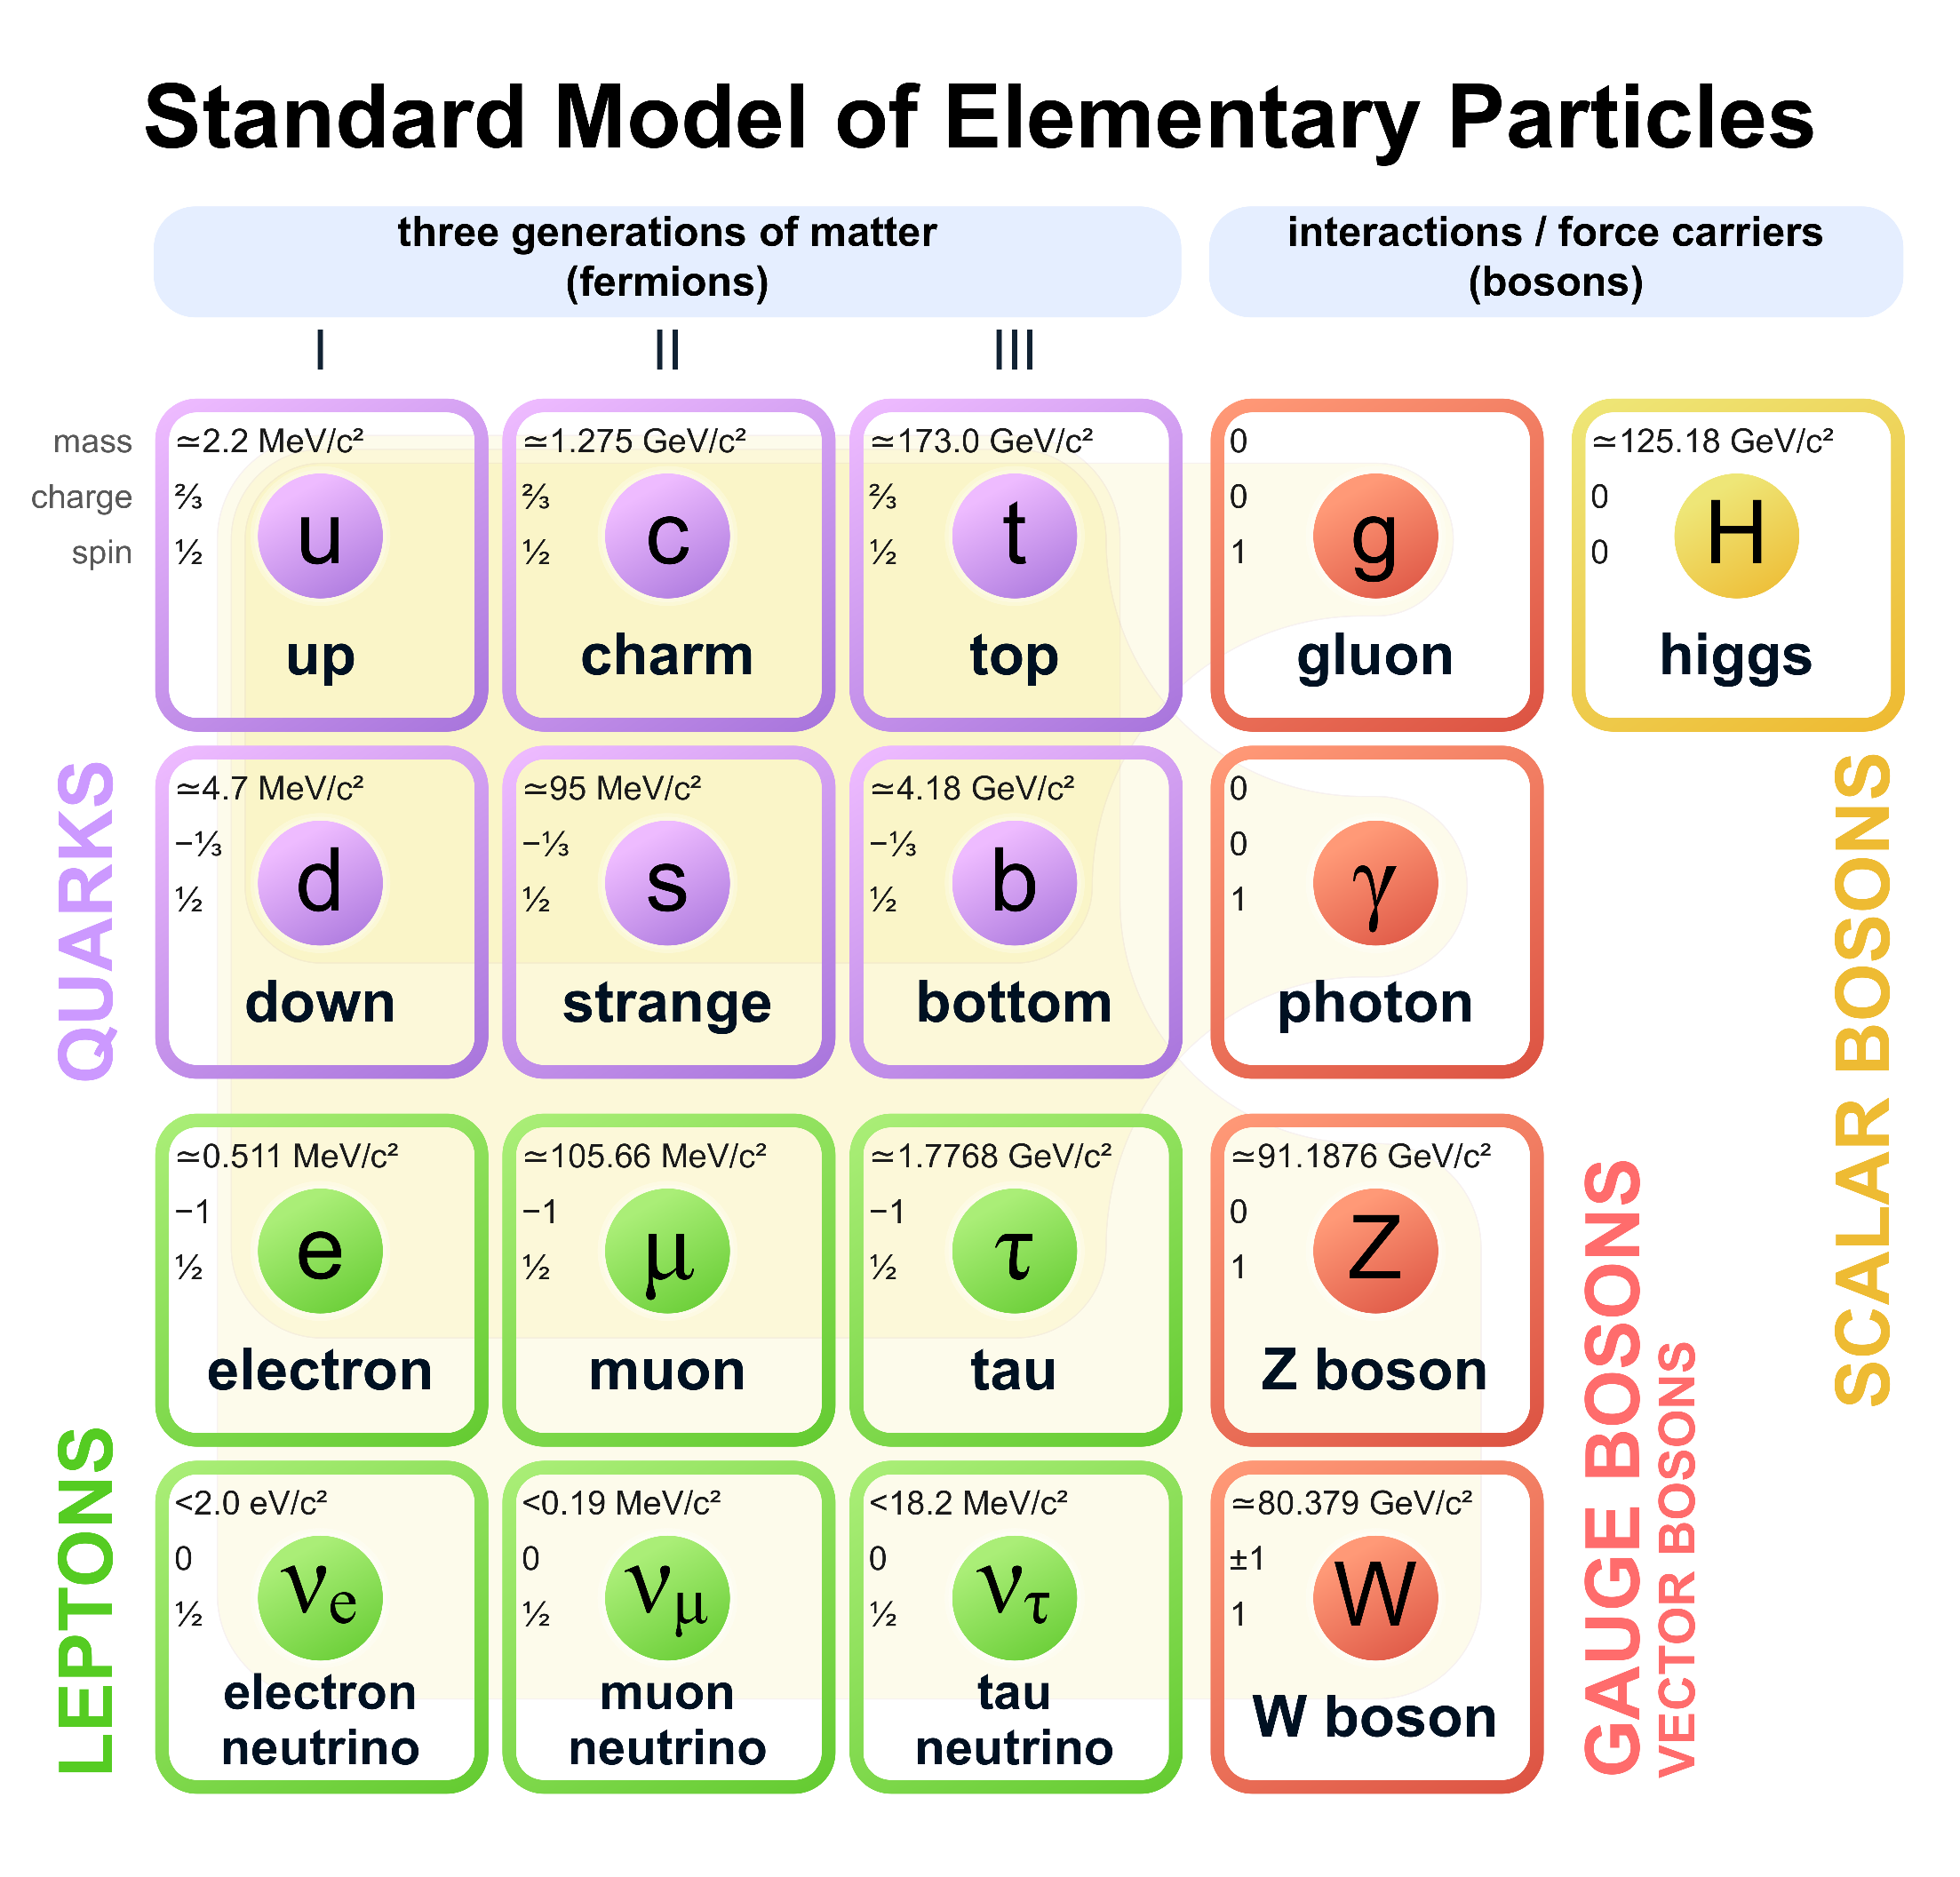
\includegraphics[width=\textwidth]{figures_SM/standard_model.eps}
	\caption[Standard Model particles]{Summary table of the Standard Model particles and their properties. The sketch~\cite{standard_model} was updated to PDG 2018 data~\cite{PDG}}
	\label{fig:sm}
\end{figure}



\subsection{Force carrier particles}

There are three interactions represented in the Standard Model of Particle Physics, the electromagnetic interaction, the weak interaction, and the strong interaction each represented by mediator bosons. The gravitation is usually not included as neither relevant at the scale of particle physics nor fully included in the model.

The electromagnetic force is described by the theory of quantum electrodynamics and couples to the electric charge of particles. Its mediator is the massless photon.

The weak force, most commonly known as the interaction of the $\beta$-decay, couples to the weak charge that every particle inherits and its mediators are the \PZ and the two opposite-charged \PW-Bosons.

The electromagnetic and the weak force can be unified as the electroweak interaction forming a $SU(2) \times U(1)$ symmetry.

The strong force responsible for the binding of quarks in the nucleons is mediated by the colour charged gluons. It only couples to particles with colour charge and is represented by the $SU(3)$ symmetry term in the Standard Model.

As already stated the gravitational force is not included in the standard model as its coupling strength at the scale is only of the order \num{10E-37}. Although it is not a mediator the Higgs boson was included in the Standard Model after its discovery in 2012.

\subsection{Matter particles}

The non-mediator particles in the model are fermions broadly classified into leptons and quarks both categorised in three generations.

The first generation of particles form the matter we see in our everyday life. The electron, the electron-neutrino and the \Pup- and \Pdown-quark as the constituents of the nucleons.
In the higher generations the defining quantum numbers stay the same while the mass of the particles increases.
Moreover there is an antiparticle for each particle with all quantum numbers reversed.

All particles interact with the weak force and only the neutrinos couple to no other interaction.
The non-neutrino leptons electron, muon, and tauon have additional electric charge and therefore also interact via the electromagnetic interaction.
The quarks are the only particles interacting with all three forces. They carry not only a weak and an electric charge but also colour charge enbaling them to interact with gluons.


\subsection{The CKM matrix}

One aspect of the standard model worth looking at in particular is the CKM matrix which describes the probability of a quark of one flavour generation to be transformed into another quark of suitable charge via the charged weak interaction namely a \PW-boson.
Each parameter $V_{ij}$ represents the probability of a transition between flavour $i$ to flavour $j$. The elements of the matrix predicted with the standard model theory show great agreement to the experimental results.~\cite{pdg}

\begin{align}
\begin{pmatrix}
\Pdown^{\prime} \\
\Pstrange^{\prime} \\
\Pbottom^{\prime}
\end{pmatrix}
&=
\begin{pmatrix}
\Vud & \Vus & \Vub \\
\Vcd & \Vcs & \Vcb \\
\Vtd & \Vts & \Vtb \\
\end{pmatrix}
\cdot
\begin{pmatrix}
\Pdown \\
\Pstrange \\
\Pbottom
\end{pmatrix}\\
%
\begin{pmatrix}
\Pdown^{\prime} \\
\Pstrange^{\prime} \\
\Pbottom^{\prime}
\end{pmatrix}
&=
\begin{pmatrix}
9.97446 & 0.22452 & 0.00365 \\
0.22438 & 0.97359 & 0.04214 \\
0.00896 & 0.04133 & 0.999105 \\
\end{pmatrix}
\cdot
\begin{pmatrix}
\Pdown \\
\Pstrange \\
\Pbottom
\end{pmatrix}
\end{align}

Important properties not listed in figure xy are the cross-section and the branching fraction.

\subsection{Top quark properties}

The most essential aspects of particle interactions needed to be understood for this thesis is the production and decay process of the \Ptop-quark. This section introduces the main properties of the top quark. Chapter XY then expands this explanation by discussing the production and decay behaviour of \Ptop- quarks in the Large Hadron Collider.

The \Ptop-quark being the up-type quark of the third generation quarks has a special standing in the field of elementary particles because its mass exceeds the other masses by \num{2} orders of magnitude. It weights about \SI{173}{\giga \electronvolt} which is higher than the masses of the weak mediators. It almost exclusively decays into a \PW and a \Pbottom quark,

\begin{align}
\frac{\Gamma_{\Ptop \rightarrow \PW \Pbottom}}{\Gamma_{\Ptop \rightarrow \PW \Pquark}} = \SI{0.957(34)}{}
\end{align},

and has a lifetime of $\mysim$ \SI{5E-25}{\second} which is smaller than the typical hadronisation time resulting in the \Ptop-quark forming no bound states.

These essential properties of the heaviest quark lead to some interesting aspects in its analysis further introduced in the following chapters.


For more information about the standard model see ~\cite{thomson, griffiths}




\section{Kinematics of collider physics}

There are a few kinematic variables and experimental properties worth discussing because the are characteristic for collider experiments which will be briefly introduced in this section.

One of the most important properties of a collider experiment is its centre-of-mass energy, \Ecms~ denoting the available energy for particle analysis offered by the experiment.
It is defined as:

\begin{align}
\Ecms = \sqrt{ \left( \sum_i E_i \right)^2 - \left( \sum_i p_i \right)^2 }
\end{align}


where $E_i$ and $p_i$ are the energies and momenta of the initial state particles.
In the case of the Large Hadron Collider used for the simulation in this thesis and introduced in chapter \ref{chp:lhc_atlas} two beams of equal beam energy are brought to collision resulting in an energy formula of

\begin{align}
\Ecms = 2 E_{beam}
\end{align}

assuming there are two beams with energies much higher than the particle's masses and therefore allowing to neglect them..

The second property is the luminosity of an experiment stating how many interactions an experiment can produce. For the colliding gaussian beams underlying the simulations in this work it can be defined as:

\begin{align}
L =f \frac{n_1 n_2}{4 \pi \sigma_x \sigma_y}
\end{align}

where $f$ is the frequency, $n_i$ is the particle number per bunch and the $\sigma_i$ values stand for the horizontal and vertical beam size respecively.
The integrated luminosity is then used to estimate the total number of interactions for a certain period of measurement:

\begin{align}
\mathcal{L} = \int L(t) dt
\end{align}

Multiplied with a cross-section the corresponding number of interactions to be expected, $N$, can be defined as $N = \sigma \mathcal{L}$.


